\section*{Assignment 5.2}

Let $X_1, \ldots, X_n$ be i.i.d. exponential random variables with parameter $\beta$. Recall that $Y = X_1 + X_2 + \cdots + X_n$ follows a Gamma distribution with parameters $\alpha = n$ and $\beta$. Transform this expression further to yield a chi-squared random variable.\\
~\\
Let $X$ be an exponential random variable with parameter $\beta$. Devise a test statistic for testing $H_0: \beta = \beta_0$ and $H_0: \beta\leq \beta_0$ in a Fisher test. \\
~\\
\textbf{\underline{Solution}.} Since $Y$ follows a Gamma distribution with parameters $\alpha = n$ and $\beta$, we have the density function
\begin{align*}
f_Y(y) = \frac{\beta^{n}}{\Gamma(n)} y^{n-1}e^{-\beta y}, \qquad y > 0
\end{align*}
and $f_Y(y) = 0$ when $y \leq 0$. Let $u = \varphi(y) = 2\beta y$, then
\begin{align*}
y = \varphi^{-1}(u) = \frac{u}{2\beta}\quad\Rightarrow\quad \frac{\U{d}}{\U{d}u}\varphi^{-1}(u) = \frac{1}{2\beta}.
\end{align*}
Then using transformation of variable, we have
\begin{align*}
f_U(u) & = f_Y\circ \varphi^{-1}(u)\cdot \left|\frac{\U{d}}{\U{d}u}\varphi^{-1}(u) \right| \\
& = \frac{\beta^n}{\Gamma(n)} \frac{u^{n-1}}{(2\beta)^{n-1}} e^{-u/2}\cdot \frac{1}{2\beta} \\
& = \frac{1}{2^{n}\Gamma(n)} u^{n-1}e^{-u/2} \qquad u > 0,
\end{align*}
and $f_U(u) = 0$ when $u\leq 0$, which is a chi-squared distribution with $2n$ degrees of freedom. Therefore, we have the distribution
\begin{align*}
Y \sim \frac{1}{2\beta} \chi_{2n}^2.
\end{align*}
Given samples $X_1, \ldots, X_n$ with size $n$, we can use test statistic
\begin{align*}
\chi_{2n}^2 = 2\beta_0 \sum_{i=1}^n X_i = 2n\beta_0 \overline{X}.
\end{align*}
With larger true parameter $\beta$, we would expect a smaller test statistic
\begin{itemize}
	\item For one-tailed test $\beta\leq \beta_0$, ``more extreme data'' means smaller $\overline{X}$. Therefore, the p-value is given by
	\begin{align*}
	P\U{-value} = F_{\chi_{2n}^2}\left(2n\beta_0\overline{X} \right),
	\end{align*}
	where $F_{\chi_{2n}^2}$ is the cumulative distribution function of chi-squared distribution with $2n$ degrees of freedom.
	\item For two-tailed test $\beta = \beta_0$, the p-value is given by
	\begin{align*}
	P\U{-value} = 2\min\left(F_{\chi_{2n}^2}\left(2n\beta_0\overline{X} \right), 1-F_{\chi_{2n}^2}\left(2n\beta_0\overline{X} \right) \right).
	\end{align*}
\end{itemize}
If we want to have a critical region for the tests, with the test statistic $\chi_{2n}^2$ defined above, we reject $H_0$ at significance level $\alpha$
\begin{itemize}
	\item $H_0: \beta = \beta_0$ if $\chi_{2n}^2 < \chi_{2n, 1-\alpha/2}^2$ or $\chi_{2n}^2 > \chi_{2n, \alpha/2}^2$,
	\item $H_0: \beta \leq \beta_0$ if $\chi_{2n}^2 < \chi_{2n, 1-\alpha}^2$,
	\item $H_0: \beta \geq \beta_0$ if $\chi_{2n}^2 > \chi_{2n, \alpha}^2$.
\end{itemize}

\section*{Critical Region and Confidence Interval}

Suppose we have a sample $X_1, \ldots, X_n$ of size $n$ from a normal population $X$ with mean $\mu$ and known variance $\sigma^2$. We would like to test the hypotheses
\begin{align*}
H_0: \mu \leq \mu_0, \qquad H_1: \mu > \mu_0.
\end{align*}
Then for such one-tailed tests, what is the corresponding confidence interval? We know that we reject $H_0$ at significance level $\alpha$ if 
\begin{align*}
Z = \frac{\overline{X} - \mu_0}{\sigma/\sqrt{n}} > z_{\alpha},
\end{align*}
which can be rewritten as
\begin{align*}
\mu_0 < \overline{X} - z_{\alpha}\frac{\sigma}{\sqrt{n}}.
\end{align*}
Since we know that if the inequality above holds, we will reject $H_0$, in which case the null value $\mu_0$ falls \underline{outside} of the confidence interval. Therefore, the corresponding confidence interval is given by
\begin{align*}
\U{CI} = \left[\overline{X} - z_{\alpha}\frac{\sigma}{\sqrt{n}}, \infty \right).
\end{align*}
Similarly, if the null hypothesis is $H_0: \mu\geq \mu_0$, the corresponding one-sided confidence interval is given by
\begin{align*}
\U{CI} = \left(-\infty, \overline{X} + z_{\alpha}\frac{\sigma}{\sqrt{n}} \right].
\end{align*}


\section*{Mean and Variance for Rank Sum}

\textbf{\underline{Wilcoxon rank-sum test statistic}.} Let $X_1, \ldots, X_m$ and $Y_1, \ldots, Y_n$, where $m\leq n$, be random samples from two continuous populations $X$ and $Y$ and associate the rank $R_i, i = 1,\ldots, m+n$, to the $R_i$th smallest among the $m+n$ total observations. The test statistic is given by
\begin{align*}
W_m = \U{sum\ of\ the\ ranks\ of\ } X_1, \ldots, X_m
\end{align*}
with
\begin{align*}
\U{E}[W_m] = \frac{m(m+n+1)}{2}, \qquad \U{Var}[W_m] = \frac{mn(m+n+1)}{12}.
\end{align*}
\textbf{\underline{Proof}.} The rank of the $m+n$ random variables follows a uniform discrete distribution. Namely,
\begin{align*}
P[R_i = k] = \frac{1}{m+n}, \qquad \U{for\ } k = 1, \ldots, m+n.
\end{align*}
Therefore, the expectation of each rank is given by
\begin{align*}
\U{E}[R_i] = \frac{1}{m+n} \sum_{k=1}^{m+n} = \frac{m+n+1}{2},
\end{align*}
giving
\begin{align*}
\U{E}[W_m] = \U{E}\left[\sum_{i=1}^m R_i \right] = \frac{m(m+n+1)}{2}.
\end{align*}
Denote $N = m + n$. We know that
\begin{align*}
\sum_{i=1}^{N} i^2 = \frac{N(N+1)(2N+1)}{6}, \qquad \sum_{i=1}^{N}\sum_{j=1}^N = \left(\sum_{i=1}^{N} i \right)^2 = \frac{N^2(N+1)^2}{4}.
\end{align*}
Therefore,
\begin{align*}
\sum_{i\neq j}^{N} ij = \frac{N^2(N+1)^2}{4} - \frac{N(N+1)(2N+1)}{6}.
\end{align*}
By properties of variance, we have
\begin{align*}
\U{Var}[W_m] & = \U{Var}\left[\sum_{i=1}^m R_i\right] = \sum_{i=1}^m \U{Var}[R_i] + \sum_{i\neq j}^m \U{Cov}[R_i, R_j],
\end{align*}
where
\begin{align*}
\U{Var}[R_i] & = \U{E}[R_i^2] - \U{E}[R_i]^2 \\
& = \frac{(N+1)(2N+1)}{6} - \left(\frac{N+1}{2} \right)^2 \\
& = \frac{N^2-1}{12}, \\
\U{Cov}[R_i, R_j] & = \U{E}[R_iR_j] - \U{E}[R_i]\U{E}[R_j] \\
& = \sum_{i\neq j}^N \frac{ij}{N(N-1)} - \left(\frac{N+1}{2} \right)^2 \\
& = \frac{N(N+1)^2}{4(N-1)} - \frac{(N+1)(2N+1)}{6(N-1)} - \frac{(N+1)^2}{4} \\
& = -\frac{N+1}{12}.
\end{align*}
Therefore,
\begin{align*}
\U{Var}[W_m] & = \sum_{i=1}^m \U{Var}[R_i] + \sum_{i\neq j}^m \U{Cov}[R_i, R_j] \\
& = \frac{m(N^2-1)}{12} - m(m-1)\cdot \frac{N+1}{12} \\
& = \frac{m(N-m)(N+1)}{12} \\
& = \frac{mn(m+n+1)}{12}.
\end{align*}

\section*{Comparison of Means}

\subsection*{Exercise 1.}

Suppose we have two normally distributed populations $X^{(1)}$ and $X^{(2)}$ with mean $\mu_1, \mu_2$ and variances $\sigma_1^2, \sigma_2^2$, respectively. A sample of size $n = 20$ is gathered for each of these populations
\begin{align*}
X^{(1)} \quad 
\begin{array}{ccccc}
3.73 & 2.90 & 2.58 & 3.33 & 3.34 \\
2.80 & 3.84 & 3.01 & 2.91 & 0.83 \\
4.54 & 3.49 & 1.12 & 0.78 & 0.67 \\
2.32 & 2.42 & 3.21 & 3.09 & 1.16
\end{array}
\end{align*}
and
\begin{align*}
X^{(2)} \quad
\begin{array}{ccccc}
1.30 & 2.55 & 3.03 & 1.71 & 2.45 \\
1.58 & 2.68 & 1.07 & 2.45 & 2.72 \\
2.54 & 2.59 & 2.35 & 2.42 & 2.87 \\
4.13 & 1.73 & 2.42 & 3.03 & 1.23
\end{array}
\end{align*}
We want to test the hypotheses
\begin{align*}
H_0: \mu_1 = \mu_2, \qquad H_1: |\mu_1 - \mu_2| \geq 0.5,
\end{align*}
with significance level $\alpha = 0.05$ in the following cases.
\begin{enumerate}
	\item We know the variances are $\sigma_1^2 = \sigma_2^2 = 1$. Perform the test. What is the required sample size for the power of the test to be at least 80\%? \\
	\textbf{\underline{Solution}.} We calculate
	\begin{align*}
	\overline{x}^{(1)} = 2.604, \qquad \overline{x}^{(2)} = 2.343.
	\end{align*}
	Then the test statistic is given by
	\begin{align*}
	z = \frac{\overline{x}^{(1)} - \overline{x}^{(2)}}{\sqrt{\sigma_1^2/n_1 + \sigma_2^2/n_2}} = \frac{2.604 - 2.343}{\sqrt{1/20+1/20}} = 0.8254.
	\end{align*}
	The critical value is given by $z_{\alpha/2} = 1.96 > z$. Therefore, we fail to reject $H_0$. We calculate
	\begin{align*}
	d = \frac{|\mu_1-\mu_2|}{\sigma} = 0.5,
	\end{align*}
	and read from OC curve for normal tests. We would require a sample size of at least 40.
	\begin{figure}[H]
		\centering
		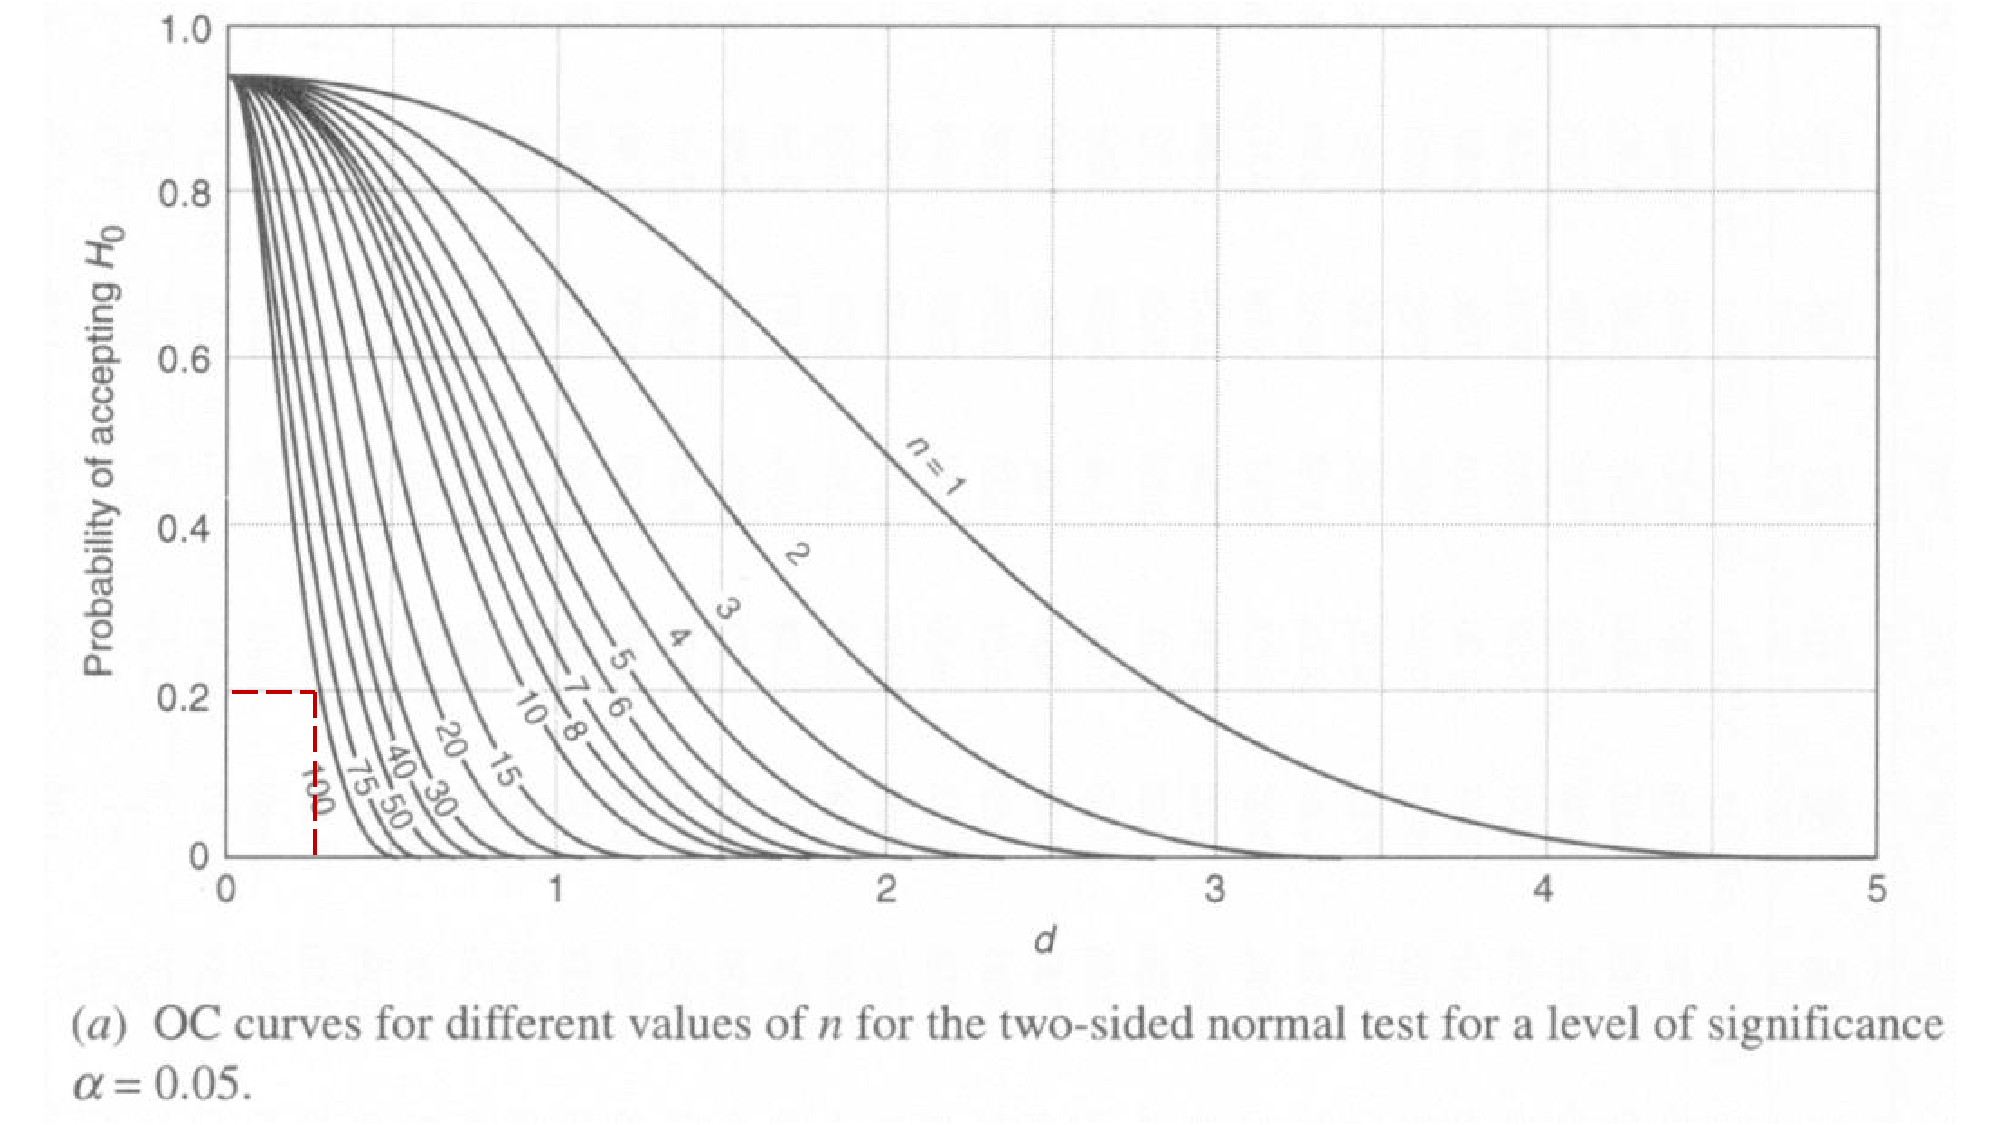
\includegraphics[width=\linewidth]{./images/s6fig1.pdf}
	\end{figure}
	\item The variances are unknown but equal $\sigma^2 = \sigma_1^2 = \sigma_2^2$. Perform the test. What is the required sample size for the power of the test to be at least 70\%? \\
	\textbf{\underline{Solution}.} We calculate the variances
	\begin{align*}
	s_1^2 = 1.263, \qquad s_2^2 = 0.534, \qquad s_p^2 = \frac{(n_1-1)s_1^2 + (n_2-1)s_2^2}{n_1+n_2-2} = \frac{s_1^2 + s_2^2}{2} = 0.899.
	\end{align*}
	Then the test statistic is given by
	\begin{align*}
	t_{38} = \frac{\overline{x}^{(1)} - \overline{x}^{(2)}}{\sqrt{s_p^2(1/n_1+1/n_2)}} = 0.871.
	\end{align*}
	The critical value is given by $t_{\alpha/2,38} = 2.024 > t_{38}$. Therefore, we fail to reject $H_0$. We calculate
	\begin{align*}
	d = \frac{|\mu_1-\mu_2|}{2s_p} = \frac{0.5}{2\sqrt{0.899}} = 0.264,
	\end{align*}
	where we estimate the variance using pooled variance, and read from OC curve for normal tests. We would require a \underline{modified sample} size of at least $n^* = 2n-1 = 75$, giving $n = 38$.
	\begin{figure}[H]
		\centering
		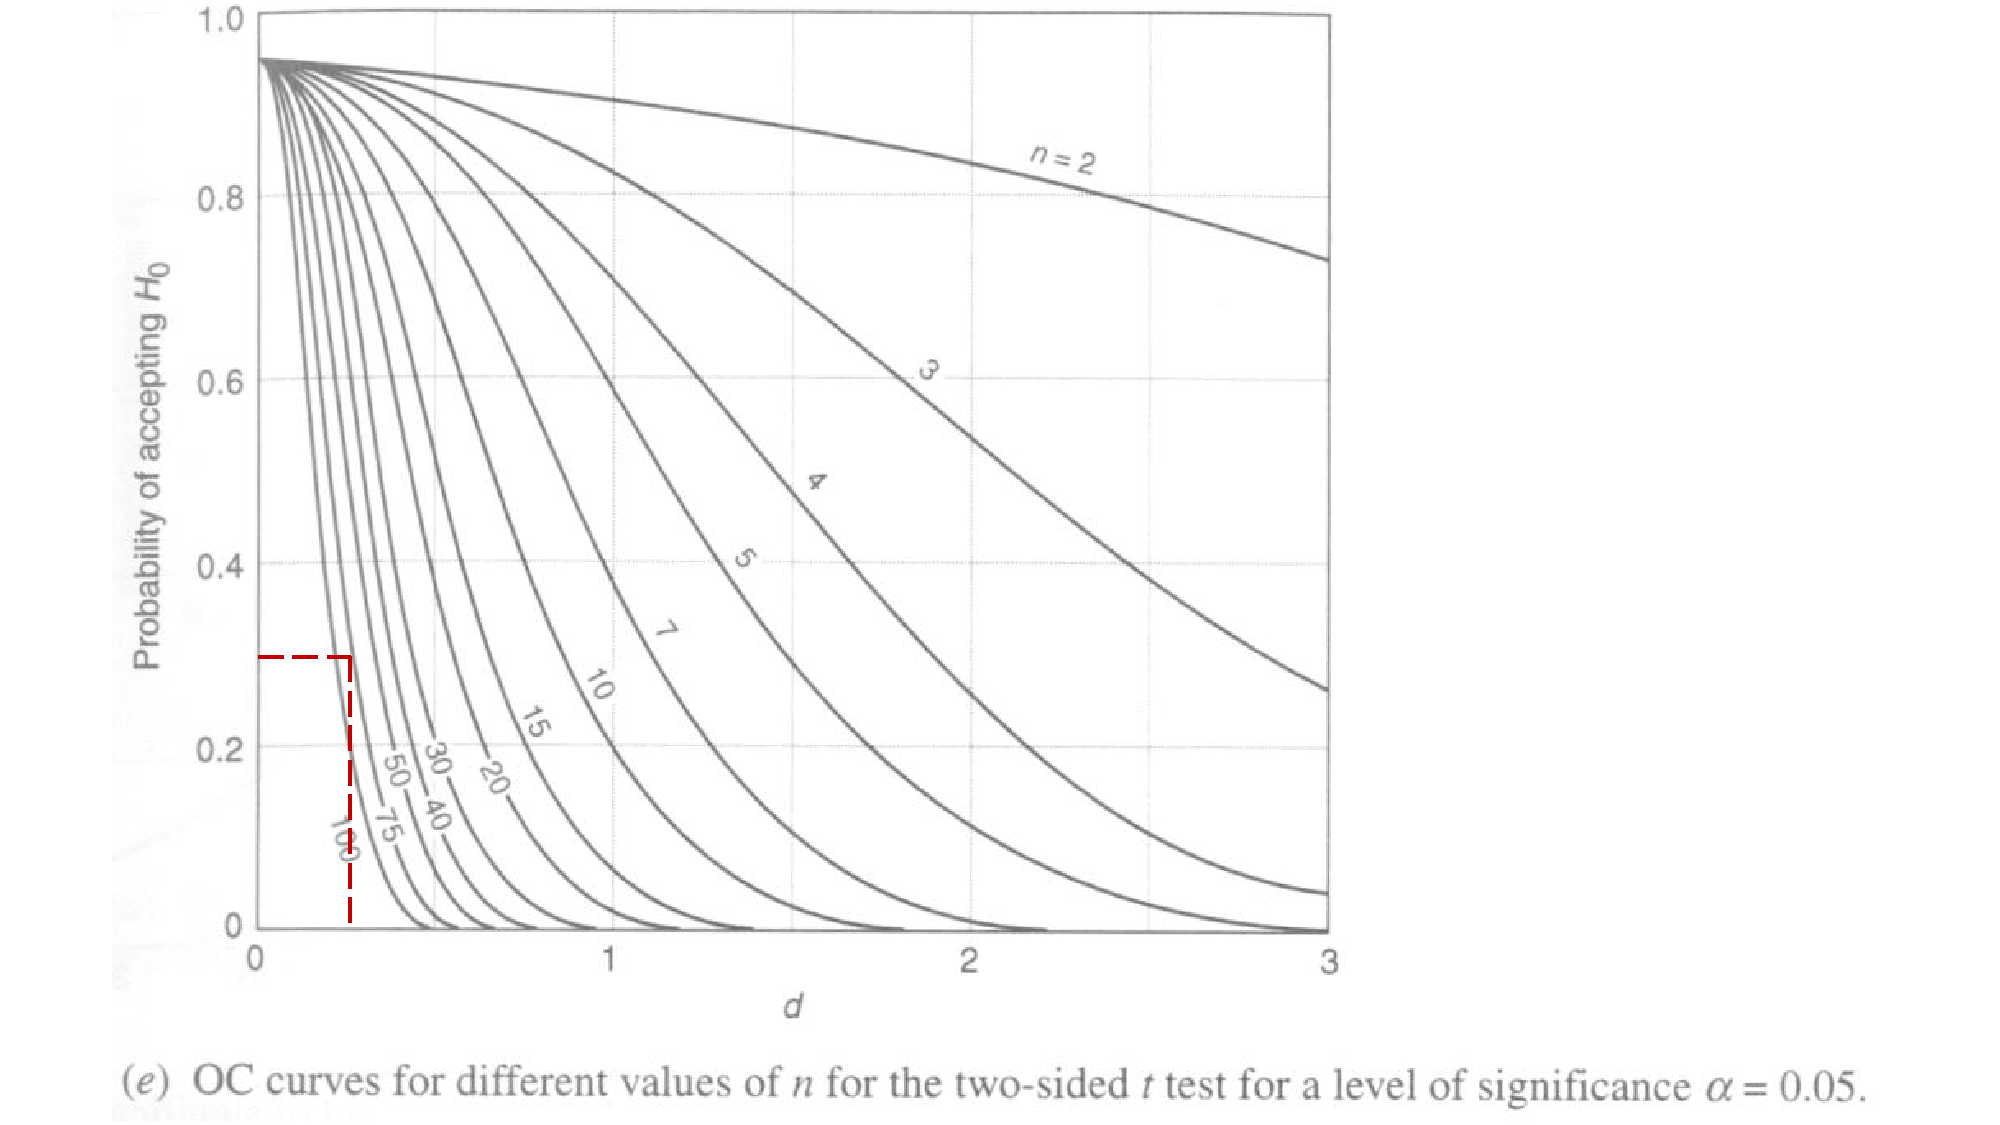
\includegraphics[width=\linewidth]{./images/s6fig2.pdf}
	\end{figure}
	\item The variances are unknown and not necessarily equal. Perform the hypothesis test. \\
	\textbf{\underline{Solution}.} We calculate
	\begin{align*}
	\gamma = \frac{(s_1^2/n_1 + s_2^2/n_2)^2}{\dfrac{(s_1^2/n_1)^2}{n_1-1} + \dfrac{(s_2^2/n_2)^2}{n_2-1}} = 32.64 \approx 32
	\end{align*}
	and thus the test statistic
	\begin{align*}
	t_{32} = \frac{\overline{x}^{(1)} - \overline{x}^{(2)}}{\sqrt{s_1^2/n_1 + s_2^2/n_2}} = 0.871
	\end{align*}
	with critical value $t_{\alpha/2, 32} = 2.04 > t_{32}$. Therefore, we fail to reject $H_0$.
\end{enumerate}



\section*{Pearson Statistic}

\subsection*{Exercise 2.}

Let $X$ denote the number of defective components from a pack of 12 such components. 100 such packs are observed, and the corresponding values of $X$ are as follows.
\begin{table}[H]
	\centering
	\begin{tabular}{c|ccccc}
		$X$ & 0 & 1 & 2 & 3 & 4 \\
		Count & 16 & 42 & 36 & 5 & 1
	\end{tabular}
\end{table}
Perform a test to analyze whether a binomial distribution is an appropriate model for the distribution of $X$. \\
~\\
\textbf{\underline{Solution}.} We set up the hypothesis
\begin{align*}
H_0: X \U{\ follows\ a\ binomial\ distribution\ with\ parameters\ } n = 12 \U{\ and\ } p,
\end{align*}
where $p$ is unknown and requires an estimate
\begin{align*}
\widehat{p} = \frac{1}{12\times 100}(42 + 2\times 36 + 3\times 5 + 4\times 1) = 0.1108.
\end{align*}
Then we calculate
\begin{align*}
P[X = 0] & = \binom{12}{0}(1-\widehat{p})^{12} = 0.244, \\
P[X = 1] & = \binom{12}{1}\widehat{p}(1-\widehat{p})^{11} = 0.365, \\
P[X = 2] & = \binom{12}{2}\widehat{p}^2(1-\widehat{p})^{10} = 0.250, \\
P[X = 3] & = \binom{12}{3}\widehat{p}^3(1-\widehat{p})^{9} = 0.104, \\
P[X \geq 4] & = 1 - P[X<4] = 0.036.
\end{align*}
Therefore, the observations and expectations can be listed as follows.
\begin{table}[H]
	\centering
	\begin{tabular}{c|ccccc}
		$X$ & 0 & 1 & 2 & 3 & 4 \\
		$O$ & 16 & 42 & 36 & 5 & 1 \\
		$E$ & 24.423 & 36.631 & 25.045 & 10.406 & 3.595
	\end{tabular}
\end{table}
We check that Cochran's rule is satisfied. The Pearson statistic is then given by
\begin{align*}
\chi_{3}^2 = \sum_{i=1}^5 \frac{(O_i - E_i)^2}{E_i} = 13.197,
\end{align*}
with critical value $\chi_{0.05,3} = 7.81 < \chi_{4}^2$ and $5 - 1 - 1 = 3$ degrees of freedom. Therefore, we reject $H_0$ with significance level 0.05. There is evidence that $X$ does not follow a binomial distribution.

